\section{Post-processing: Reading a show file and computing some Aerodynamic Quantities}
\index{post processing}\index{lift}\index{drag}

The program {\tt bin/aero.C} shows how to read a show file that has been
generated by \solver\ and access the solution values stored there. This program
can then be used to plot the pressure coefficient on the surface of a body
and to compute the lift and drag on a body. 

The file {\tt aero.C} can be altered to compute other quantities that may
be of particular interest to your application. All information about the grid,
solutions and cgins parameters are accessible from the show file. You could, for example
use this program to output the solution values to a data file format suitable for some
other plotting or analysis program.

\begin{figure}[hb]
\begin{center}
%%  \epsfig{file=\obFigures/aero.naca.cp.ps,width=.8\linewidth}  \\
  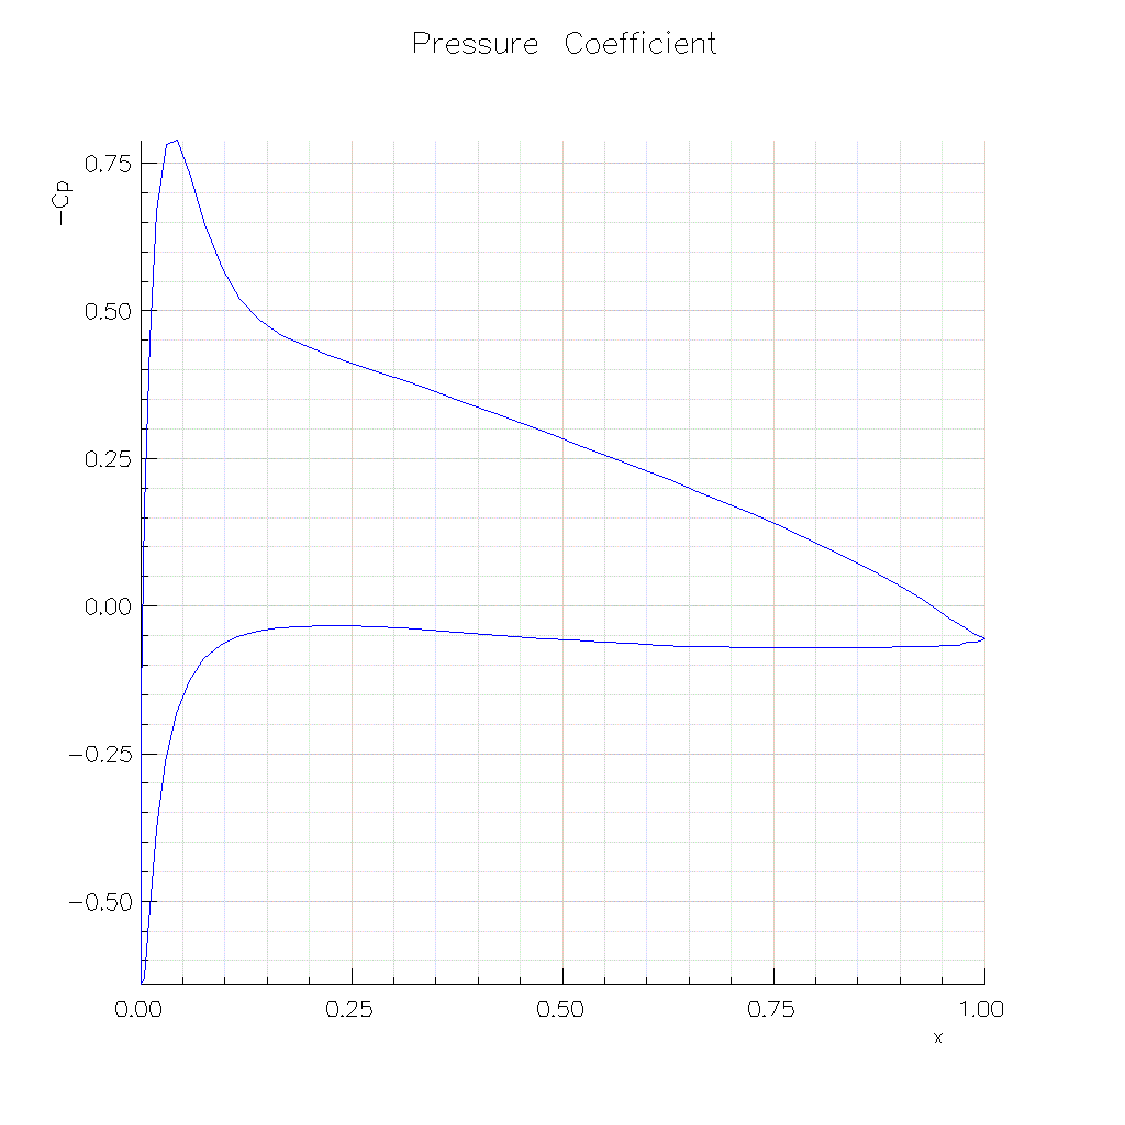
\includegraphics[width=.8\linewidth]{\insDocDir/fig/aero_naca_cp}
 \caption{The areo.C program can be used to read a show file generated by cgins and compute
the coefficient of pressure on the surface of a body.}
\end{center}
\end{figure}

